\documentclass{article}

\usepackage[final]{neurips_2019}
\usepackage{symbols}
\usepackage[utf8]{inputenc} % allow utf-8 input
\usepackage[T1]{fontenc}    % use 8-bit T1 fonts
\usepackage{hyperref}       % hyperlinks
\usepackage{url}            % simple URL typesetting
\usepackage{booktabs}       % professional-quality tables
\usepackage{amsfonts}       % blackboard math symbols
\usepackage{nicefrac}       % compact symbols for 1/2, etc.
\usepackage{microtype}      % microtypography
\usepackage{amsmath}
\usepackage{amssymb}
\usepackage{graphicx}
\usepackage{xcolor}
\usepackage[ruled]{algorithm2e}

\title{Getting started with Graph Neural Networks}

\author{
  Antoine~Moulin\\
  Mathematics, Vision, Learning (MVA)\\
  ENS Paris-Saclay\\
  \texttt{antoine.moulin@ens-paris-saclay.fr}\\
  \And
  Claire~Vernade\\
  DeepMind, UK\\
  \texttt{claire.vernade@gmail.com}\\
  \And
  Rémy~Degenne\\
  CWI Amsterdam\\
  \texttt{remydegenne@gmail.com}\\
}

\begin{document}

\maketitle


% Abstract --------------------------------------------
\begin{abstract}
    Graph Neural Networks (GNNs) are models that operate on graph-structured data. In recent years, it became a very active area of research: many models have been developed and it has been used in different fields, such as computer vision, chemistry, and others. Here, we focus on the paper \cite[Battaglia et al. 2018]{battaglia2018relational}, which aims to gather many different approaches under a common framework. The authors introduce the so-called \emph{graph network} block, designed to be the building block for learning from relational data in deep learning architectures. It is based on three principles: flexible representations of the data, a configurable within-block structure to control the information made available to the different functions, and composable multi-block architectures so that different blocks can be combined to construct complex models. We start by stating some definitions and challenges any graph neural network model faces. Then, we highlight the main differences with the previous frameworks and finally, we focus on an example and applications.
\end{abstract}



% Introduction ----------------------------------------
\section{Introduction}
\label{sec:introduction}

A graph is a data structure used to represent \emph{relations} between different \emph{entities}. For instance, a mass-spring system can be seen as a graph where nodes are the different masses and edges are the springs that connect pairs of nodes. For a social network, nodes correspond to the users, and edges represent friendships (in which case the graph is undirected, such as Facebook) or follower relationships (in which case the graph is directed, such as Twitter). Another example is given by molecules - which can be naturally seen as graphs - where nodes are the atoms and edges are the interactions between atoms.

There is an increasing amount of data generated from complex processes that cannot fit into a Euclidean representation, and for which graphs are well suited. From scene understanding to molecules classification problems, graph-related techniques are being broadly applied. After the success of deep learning in computer vision and other fields, deep learning architectures for graphs are now being developed. Besides, the previous examples show that one can face different kinds of problems. When dealing with a mass-spring system, one could be interested in predicting future positions of the masses, i.e. solving a node regression task. With a social network, link prediction can be of great interest, which corresponds to an edge classification task. Finally, being able to tell whether or not a molecule is likely to be a drug corresponds to a graph classification task.

GNNs have been first introduced with \cite[Gori et al. 2005]{gori2005GNN}. In these original works, the authors propose an extension of recursive neural networks that can be applied to any graph. Based on a dynamical system, they update the node states until it converges (which is theoretically guaranteed because a contracting mapping is used). The constraints induced by the contracting mapping raised some issues, but the main idea was here: develop a model that directly process a graph and learn some function of the nodes by iteratively propagating and aggregating information through the graph. Since then, this area of research has been growing quickly: GNNs have been used in many different contexts (see section \ref{sec:example-applications}) and plenty of versions have been developed, often with impressive results.

Here, we focus on \cite[Battaglia et al. 2018]{battaglia2018relational} (the notations used are those in the paper) and some of the ideas proposed afterward. In section \ref{sec:def-challenges}, we give some definitions and the main challenges one has to deal with when building a GNN. In section \ref{sec:background-otherworks}, we present the background on which \cite[Battaglia et al. 2018]{battaglia2018relational} is based and some other works. In section \ref{sec:framework} is exposed the framework from \cite[Battaglia et al. 2018]{battaglia2018relational} with the \emph{graph network} block and its different components. Besides, it will be linked to the previous section. Finally, in section \ref{sec:example-applications} are presented some examples and applications.



% Definitions and challenges --------------------------
\section{Definitions and challenges}
\label{sec:def-challenges}

    \subsection{Graph}
    \label{subsec:def-graph}

Before diving into the formalism of the GN block, let's give the definition of a graph that we will be using here (which can be found in \cite{battaglia2018relational}). By \emph{attribute}, we mean "properties that can be encoded as a vector, set, or even another graph". A \emph{graph} is a tuple $G = \left( \uv, V, E \right)$ such that:

\begin{itemize}
    \item[-] $G$ has a global attribute $\uv$.
    
    \item[-] $G$ has attributed vertices $V = \left\{ \vv_k \right\}_{k=1:N^v}$.
    
    \item[-] $G$ has directed, attributed edges $E = \left\{ \left( \ev_k, r_k, s_k \right) \right\}_{k=1:N^e}$ where $r_k, s_k$ are the indices of the receiver and the sender, respectively.
    
    \item[-] $G$ is a multi-graph, i.e. there can be more than one edge between vertices, including self-edges.
\end{itemize}

In the following, unless it is specified, a graph is defined like that. An illustration is given in figure \ref{fig:def-graph}. Besides the examples given in section \ref{sec:introduction}, a graph could also represent a road network between different towns. The nodes would be the towns across a country, and the edges would be the roads between them. Then, the task could be to find the shortest path between two towns. In this case, the node attributes could be for instance a position or a boolean indicating if a node is the beginning or the end of the path to find. The edge attributes could be the distances between two nodes. This example is detailed in section \ref{sec:example-applications}.

\begin{figure}
    \centering
    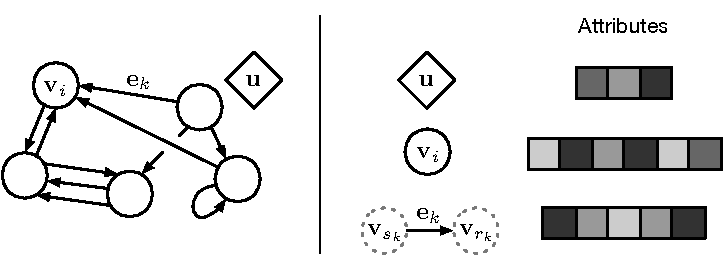
\includegraphics{images/attributes.pdf}
    \caption{An example of graph as defined in section \ref{subsec:def-graph}. (Illustration from \cite{battaglia2018relational}.)}
    \label{fig:def-graph}
\end{figure}

    \subsection{Permutation invariance and isomorphism}
    \label{subsec:perm-invariance}

Some deep learning architectures can encode spatial translation invariance (such as Convolutional Neural Networks that use the same filters on all the pixels of an image) or temporal translation invariance (such as Recurrent Neural Networks whose recurrent unit is shared over time). One of the motivations of graph neural networks is that in many cases, the objects involved in a learning task do not have a natural order (how could we order the towns from the previous example?) and that there is no deep learning model that has some kind of permutation invariance. If one trains a model using some features $\left( \xv_1, \dots, \xv_n \right)$ and that a new input has an ordering $\left( \xv_n, \xv_2, \dots, \xv_{n-1} \right)$, the model may completely fail. Similarly, if one indexes the nodes of a graph in two different ways, it will yield two different adjacency matrices, which can be an issue. Hence, we introduce the notion of equivariance and invariance functions.

For an order-$k$ tensor $T \in \mathbb{R}^{n^k}$ and $\sigma \in \mathcal{S}_n$, we define the operation: $\left( \sigma \star T \right)_{\sigma(i_1), \dots, \sigma(i_k)} = T_{i_1, \dots, i_k}$, which permutes the indices along each axis of the tensor $T$ with the same permutation $\sigma$.

\begin{itemize}
    \item[-] A function $f: \mathbb{R}^{n^k} \rightarrow \mathbb{R}^l$ is said to be \emph{invariant} if $f \left( \sigma \star T \right) = f \left( T \right)$, i.e. if the output does not depend on the input's ordering.
    
    \item[-] A function $f: \mathbb{R}^{n^k} \rightarrow \mathbb{R}^{n^l}$ is said to be \emph{equivariant} if $f \left( \sigma \star T \right) = \sigma \star f \left( T \right)$, i.e. if the output's ordering remains the same than the input's ordering, even in case of a permutation.
\end{itemize}

A graph $G$ can be seen as a $2$-tensor using the adjacency matrix $A \in \mathbb{R}^{N^v \times N^v}$ that contains $N^e$ nonzero elements. Denote by $X \in \mathbb{R}^{N^v \times d}$ the vertices' attributes. Let $P$ be a permutation matrix. In this case, the definitions can be reformulated as: $f$ is invariant if $f \left( PAP^T, PX \right) = f \left( A, X \right)$, and $f$ is equivariant if $f \left( PAP^T, PX \right) = P f \left( A, X \right)$. With these definitions in mind, we notice that when performing graph-level tasks, a GNN has to be invariant. When performing node-level tasks, a GNN has to be equivariant.

Besides, we say that two graphs $G_1$ and $G_2$ are \emph{isomorphic} if there exists $\sigma$ such that $G_1 = \sigma \star G_2$. An important question is which graphs can GNNs distinguish, and what does this depend on? While the performance of a GNN depends on its update and aggregation functions (see section \ref{sec:framework}), it has been shown in \cite[Xu et al. 2019]{xu2019powerful} that an upper bound is given by the Weisfeiler-Lehman graph isomorphism test, which we quickly define here.

Given two graphs $G$ and $G'$ (for which we assume to have generated some labels for the nodes, if not available), we would like to know whether or not $G$ and $G'$ are isomorphic. The key idea of the Weisfeiler-Lehman test is to iteratively (i) update the node labels using the sorted set of neighboring node labels, (ii) naming it as a new label. We iterate this process until the label sets of $G$ and $G'$ differ or the number of iterations reaches the number of nodes, in which case either the graphs are isomorphic, either the test failed to discriminate them. An iteration is showed in figure \ref{fig:weisfeiler-lehman}.

\begin{figure}
    \centering
    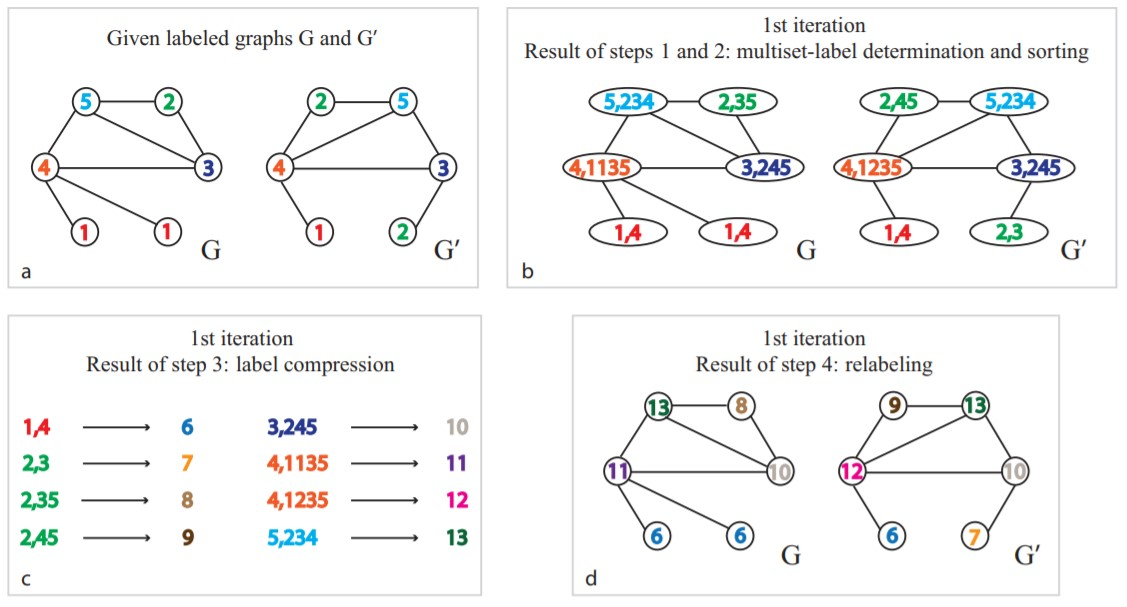
\includegraphics[scale=.58]{images/weisfeiler_lehman_iteration.jpg}
    \caption{One iteration of the Weisfeiler-Lehman graph isomorphism test. Note that here, one iteration is enough to see that $G$ and $G'$ are not isomorphic. (Illustration from \cite{shervashidze2011WeisfeilerLehmanGK}.)}
    \label{fig:weisfeiler-lehman}
\end{figure}

    \subsection{Convolution on a graph}
    \label{subsec:convolution-graph}

Given the success of CNNs, there have been some researches about how to apply a convolution on a graph. The goal for GNNs is to find a way to efficiently use the local information available in a node's neighborhood. Unlike an image that can be represented as a 2D-grid, there is no notion of space in a graph, and the neighborhood's size can vary. Different ideas were proposed. Some are designed as "spectral" methods as they rely on a computation that involves the Fourier transform of a graph signal (and thus the eigendecomposition of the Laplacian matrix). Those methods require to compute the eigendecomposition of the Laplacian matrix for each graph and thus are computationally expensive. Hence, we do not give more details about them and instead focus on "spatial" methods.

\begin{figure}
    \centering
    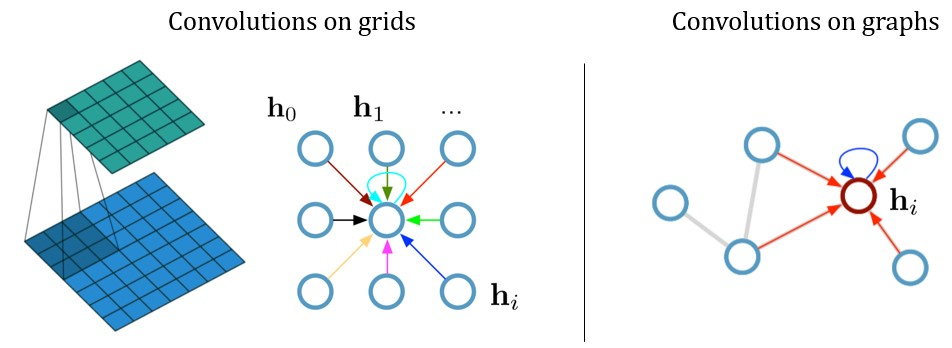
\includegraphics[scale=.6]{images/convolutions_grid_graph.jpg}
    \caption{Convolution on a grid and its possible extension on a graph. Note that while the weights corresponding to the neighbors on a grid are all different, they are shared across neighbors on a graph. $\hv_i \in \mathbb{R}^d$ are the hidden layer activations of a pixel or a node. (Illustration from Thomas Kipf.)}
    \label{fig:convolution-grid-graph}
\end{figure}

As a reminder and using notations from figure \ref{fig:convolution-grid-graph}, a convolution on the node $\hv_4 \in \mathbb{R}^d$ from a grid can be performed as:
\begin{equation*}
    \hv_4' = \sigma \left( \textcolor[rgb]{0.58, 0.07, 0.00}{\Wm_0 \hv_0} + \textcolor[rgb]{0.31, 0.56, 0.00}{\Wm_1 \hv_1} + \dots +  \textcolor{blue}{\Wm_9 \hv_9} \right)
\end{equation*}

A convolution on a graph, can be performed as:
\begin{equation*}
    \hv_i' = \sigma \left( \textcolor{blue}{\Wm_0 \hv_0} + \textcolor{red}{\Wm_1 \sum_{j \in \mathcal{N}_i} \hv_j} \right)
\end{equation*}

where $\sigma$ is a nonlinear function. Note that because of the sum, this convolution does not depend on the neighbors' order. There are many variants (e.g. using an attention mechanism) but the idea remains the same: update the node embeddings, aggregate it (here with the sum), and so on.


% Background ------------------------------------------
\section{Background and other works}
\label{sec:background-otherworks}

    \subsection{Background}
    \label{subsec:background}

Many papers proposed different approaches for GNNs before \cite[Battaglia et al. 2018]{battaglia2018relational}. Here, we only present the one from \cite[Gilmer et al. 2017]{gilmer2017neural}, which was already an attempt of unification and which will appear as a particular case of the framework mentioned here in the section \ref{sec:framework}.
    
            \subsubsubsection{\textbf{Message-Passing Neural Networks (MPNNs).}}

MPNNs were defined in \cite[Gilmer et al. 2017]{gilmer2017neural} as a class of models that learn a message-passing algorithm and an aggregation procedure to compute a function of an entire input graph. The goal was to predict properties of molecules much faster than Density Functional Theory (DFT), which is usually used in chemistry for approximations. This framework unifies different approaches, such as \cite[Kipf et al. 2016]{kipf2016semisupervised}'s one.

Let $G$ be a graph. The forward pass has two phases, a \emph{message-passing} phase and a \emph{readout} phase:

\begin{itemize}
    \item The message-passing phase runs for $T$ time steps and uses message functions $\phi_t^e$ and vertex update functions $\phi_t^v$, where $t$ stands for the time step. During this phase, the vertices' features $\vv_i$ are updated ($\vv_i^{(0)} \triangleq \vv_i$), based on messages coming from the neighborhoods and through the edges as:
    
    \begin{equation*}
        \begin{aligned}
        m_i^{t+1} &= \sum_{k:r_k=i} \phi_t^e \left( \ev_k, \vv_{r_k}^{(t)}, \vv_{s_k}^{(t)} \right) \triangleq \rho^{e \rightarrow v} \left( E_{i}^{(t)} \right) & \text{where } E_{i}^{(t)} = \left\{ \left( \ev_k, r_k, s_k \right) \right\}_{r_k=i} \\
        \vv_{i}^{(t+1)} &= \phi_t^v \left( \vv_{i}^{(t)}, m_i^{(t+1)} \right) &
        \end{aligned}
    \end{equation*}
    
    In other words, here, the edges are just a way for the vertices to communicate information, and the information is aggregated with the summation operator.
    
    \item The readout phase computes a feature vector for the whole graph using some readout function $\phi^u$ according to
    
    \begin{equation*}
        \uv = \phi^u \left( \left\{ \vv_k^{(T)} \right\}_{k=1:N^v} \right)
    \end{equation*}
\end{itemize}

The functions $\phi$ are all learned and differentiable. As $\phi^u$ operates on the set of vertices' features, it must be invariant to permutations in order for the MPNN to be invariant to graph isomorphism (see section \ref{sec:def-challenges}).

\begin{figure}[h]
    \centering
    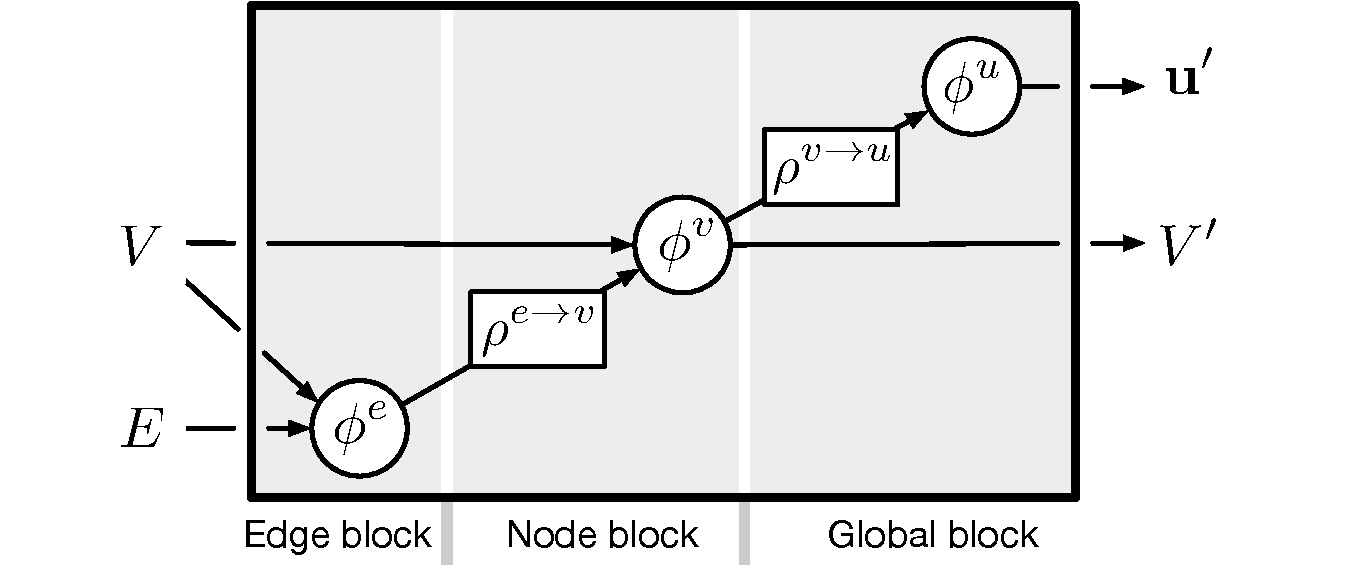
\includegraphics[scale=.5]{images/GN-mpnn-block.pdf}
    \caption{MPNN block. (Illustration from \cite{battaglia2018relational}.)}
    \label{fig:mpnn}
\end{figure}


    \subsection{Other works}
    \label{subsec:other-works}

Besides MPNNs, many different approaches have been proposed. For instance, \cite[Kipf et al. 2016]{kipf2016semisupervised} introduced a Laplacian based method, which falls in the "spectral" methods category mentioned before. \cite[Veličković et al. 2017]{velikovi2017graphattention} presents a model in which the update uses an attention mechanism. Non-Local Neural Networks from \cite[Wang et al. 2017]{wang2017nonlocal} take inspiration from the non-local mean operation.

For a more complete list, one can check the recent review from \cite[Wu et al. 2019]{wu2019comprehensive}.

% Framework ---------------------------------------
\section{The framework: Graph Network (GN)}
\label{sec:framework}

As said previously, \cite[Battaglia et al. 2018]{battaglia2018relational} introduces a general framework, the \emph{graph network} (GN) block, unifying several approaches (such as MPNNs or NLNNs). It leverages every step of the computation by formulating it in a general form, enabling anyone to custom and synthesize new architectures that express a strong relational inductive bias. In other words, this paper does not introduce a new graph-related technique strictly speaking but highlights all possible degrees of freedom in an architecture using GN blocks.

The GN block is a graph-to-graph module, based on three design principles:

\begin{itemize}
    \item \textbf{Flexible representations}. The global, node, and edge attributes of a GN block can be represented with arbitrary formats, such as sets, sequences or graphs. Most of the time however, vectors or tensors are used (one per edge or node, and one for the global attribute) so a GN can be used with other blocks such as a CNN or a RNN. Besides, when representing the input data as a graph, there are two possibilities: (i) the input explicitly specifies the structure, (ii) it must be inferred or assumed. In the second case, if the entities (i.e. the nodes) are not explicit, they can be for example inferred by a neural network. If the relations (i.e. the edges) are not explicit, one can use a fully-connected graph or try inferring sparse relations between the nodes (sparsity is often desirable, especially with graphs where it can speed up the computations).
    
    \item \textbf{Configurable within-block structure}. The structure and functions within a GN block can be configured in different ways, which offers flexibility in what information is made available as inputs to its functions, as well as how output edge, node, and global updates are produced. The different functions within a GN block are explained in this section. An illustration of the general GN block is given in figure \ref{fig:full-gn-block}, and an illustration of a MPNN, which can be seen as a particular case, is given in figure \ref{fig:mpnn}.
    
    \item \textbf{Composable multi-block architectures}. The third principle of GNs is that it must be composable so that one can build complex architectures. The graph-to-graph interface ensures that the output of one GN block can be passed as input to another, even if their internal configurations are different. This allows arbitrary numbers of GN blocks to be composed. They can also be used within a CNN or RNN architecture. Besides, the blocks can be shared (as in unrolled RNN) or not. 
\end{itemize}

Now, let's explain the structure of a GN block. It contains three "update" functions, $\phi$, and three "aggregation" functions, $\rho$. $\phi^e$ is used for the per-edge updates, $\phi^v$ for the per-node updates and $\phi^u$ for the global attribute update. $\rho^{e \rightarrow v}$ is used to aggregate information from the edges and sends it to the nodes, $\rho^{e \rightarrow u}$ serves a similar purpose but sends information to the global attribute, and $\rho^{v \rightarrow u}$ aggregates information from the nodes and sends it to the global attribute:
\begin{equation*}
    \begin{aligned}
    \ev_k' &= \phi^e \left( \ev_k, \vv_{r_k}, \vv_{s_k}, \uv \right) &\hspace*{5mm} \bar{\ev}_i' = \rho^{e \rightarrow v} \left( E_i' \right) &\hspace*{5mm} \bar{\ev}' = \rho^{e \rightarrow u} \left( E' \right) \\
    \vv_i' &= \phi^v \left( \bar{\ev}_i', \vv_i, \uv \right) &\hspace*{5mm} \bar{\vv}' = \rho^{v \rightarrow u} \left( V' \right) & \\
    \uv' &= \phi^u \left( \bar{\ev}', \bar{\vv}', \uv \right) & &
    \end{aligned}
\end{equation*}

where $E_i' = \left\{ \left( \ev_k', r_k, s_k \right) \right\}_{r_k=i, k=1:N^e}$, $E' = \left\{ \left( \ev_k', r_k, s_k \right) \right\}_{k=1;N^e}$ and $V' = \left\{ \vv_k' \right\}_{k=1:N^v}$. Note that the functions $\rho$ must be invariant to permutations. Under this form, the procedure for an update is as follows:

\begin{enumerate}
    \item Compute the per-edge updates $\ev_k'$ with the function $\phi^e$, which could correspond to the estimated time to get from one town to another (e.g. depending on the traffic). Then aggregate the information for every receiver node with the function $\rho^{e \rightarrow v}$ (e.g. a driver looks at the possible directions and choose to take the quickest route) and the message for the global attribute with the function $\rho^{e \rightarrow u}$ (e.g. the total estimated time or distance between two towns).
    
    \item Compute the per-node updates $\vv_i'$ with the function $\phi^v$, using both the current nodes' attributes and the edge messages (i.e. the $\bar{\ev}_i'$). For instance, this update could give a piece of information about whether or not the driver will have to go through a certain town. Then aggregate the new attributes with the function $\rho^{v \rightarrow u}$ to send a message to the global attribute (e.g. the number of towns to go through).
    
    \item Compute the global attribute update $\uv'$ with the function $\phi^u$, using the current global attribute, the message from the edges $\bar{\ev}'$ and the message from the nodes $\bar{v}'$.
\end{enumerate}

An illustration of such a procedure is given in figure \ref{fig:full-gn-block}. The given order is arbitrary and can be changed, i.e. one could have started to compute the per-node updates and used a function $\rho^{v \rightarrow e}$.

\begin{figure}
    \centering
    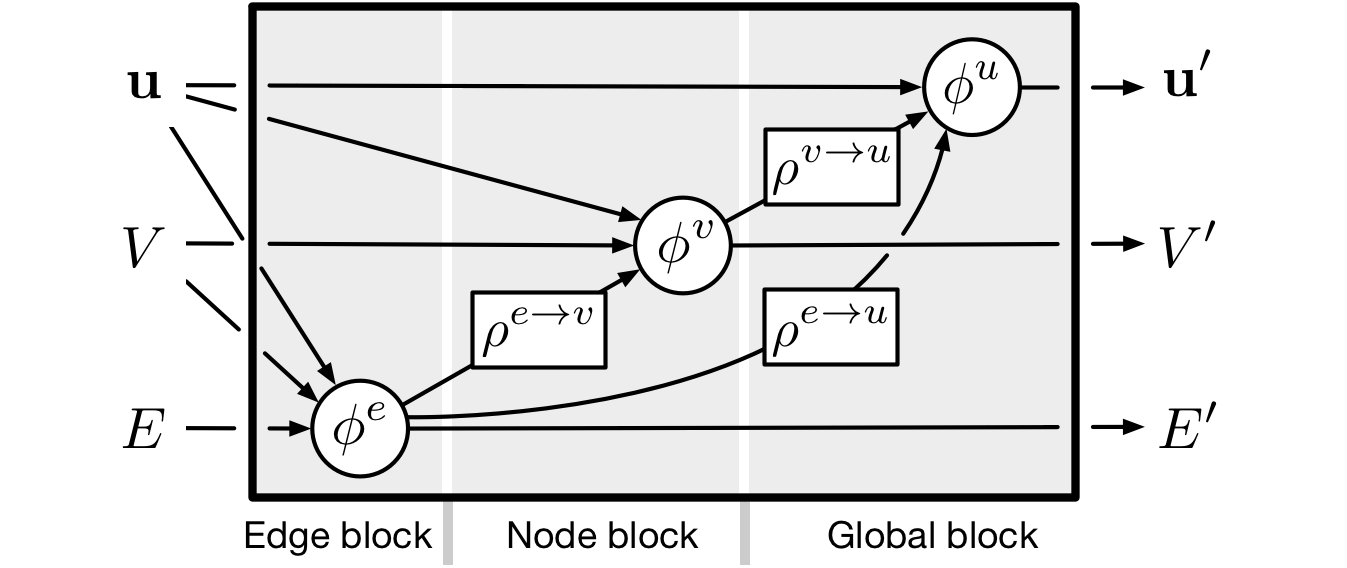
\includegraphics[scale=.5]{images/GN-full-block.png}
    \caption{A full GN block. Every degree of freedom is illustrated in this block. The $\rho$ functions must be invariant to permutations, and the $\phi$ functions can be neural networks, such as MLPs. (Illustration from \cite{battaglia2018relational}.)}
    \label{fig:full-gn-block}
\end{figure}

Other examples than MPNNs can be found in \cite{battaglia2018relational} and have different structures than showed in figure \ref{fig:mpnn}, but what we see with figures \ref{fig:mpnn} and \ref{fig:full-gn-block} is that \cite{battaglia2018relational} highlights all the possible configurations of a network that can process graphs and packs everything in an easy-to-use block, i.e. the authors present a model compatible with the current deep learning frameworks.



% Examples ---------------------------------------
\section{Example and applications}
\label{sec:example-applications}

    \subsection{Shortest path problem}
    \label{subsec:shortest-path}

Let's consider the shortest path problem. The code is available at \href{https://tinyurl.com/gn-shortest-path-demo}{\textcolor{blue}{https://tinyurl.com/gn-shortest-path-demo}} and comes from the demonstrations of the \texttt{graph\_nets} \footnote{\href{https://github.com/deepmind/graph_nets}{\textcolor{blue}{https://github.com/deepmind/graph\_nets}}} library. Let's define the GNN, step by step.

        \subsubsection{The graph}

The graphs are generated as follows: (i) $N^v$ nodes are uniformly sampled in a 2D rectangle, (ii) $N^v$ weights are sampled according to an exponential law and assigned to each node, (iii) edges are generated according the geographical threshold model (which just says that two nodes are connected if their weights verify a certain relation) and (iv) the graph is combined with a minimum spanning tree to ensure the graph is connected.

Here, the edges have two attributes represented in an array:
\begin{itemize}
    \item \texttt{distance}, which gives the Euclidean distance between two nodes,
    \item \texttt{solution}, which is a boolean to be determined and indicates if the edge belongs to the predicted path. The second attribute is not necessary, as it will be in the nodes as well, but shows that edge classification can be done.
\end{itemize}

The nodes have five attributes represented in an array:
\begin{itemize}
    \item \texttt{pos}, which gives the position of a node in $\mathbb{R}^2$,
    \item \texttt{weight}, which has been sampled from an exponential law,
    \item \texttt{start}, which indicates if the node is the source of the path,
    \item \texttt{end}, which indicates if the node is the target one wants to reach,
    \item \texttt{solution}, which indicates if the node belongs to the path (to be determined).
\end{itemize}

And the global attribute can be defined as the length of the path, which is stored in an array as well.
        \subsubsection{The within-block structure}
        
Within each block of the model used, the update functions $\phi^e, \phi^v$ and $\phi^u$ are all defined as a Multi-Layer Perceptrons (MLPs) with two hidden layers that contain 16 hidden units each. They have to be trained.

The aggregate functions $\rho^e, \rho^v$ and $\rho^u$ are all defined as the sum operator.
        
        \subsubsection{The configuration}

The configuration of the GNN is an autoencoder formed by three components:
\begin{itemize}
    \item an encoder, which learns an embedding for the nodes, edges and the global attribute,
    \item a core module that performs several message-passing phases with the encoder's output and a hidden state, in a recurrent fashion,
    \item a decoder, which decodes the output of the code module.
\end{itemize}

The core module is where the problem is solved. The configuration is showed in figure \ref{fig:GN-rnn-config}.

\begin{figure}
    \centering
    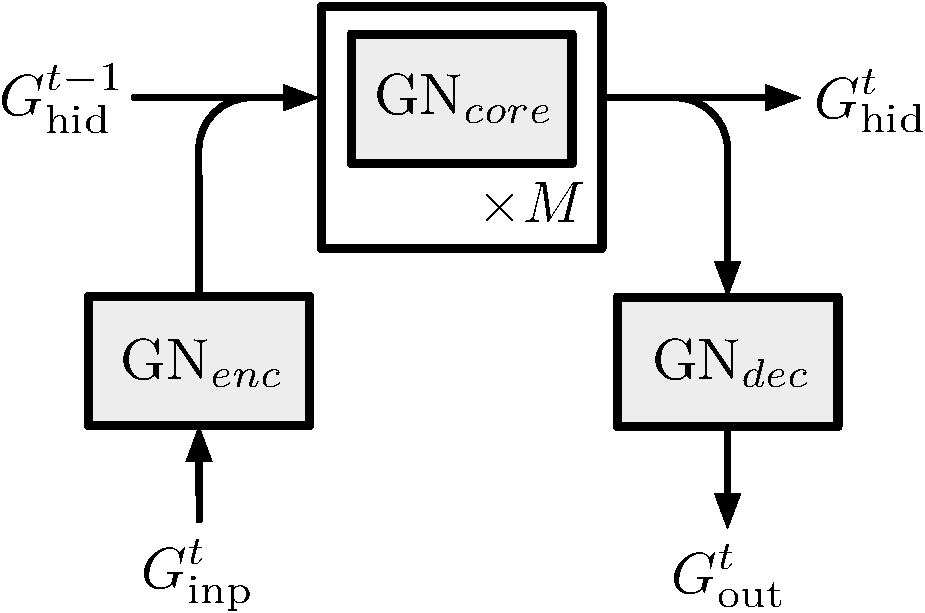
\includegraphics[scale=.4]{images/GN-rnn-config.pdf}
    \caption{Configuration of the GNN used for solving the shortest path problem. (from \cite{battaglia2018relational}.)}
    \label{fig:GN-rnn-config}
\end{figure}

        \subsubsection{Analysis}

After around 2000 iterations of training, the GNN reaches around 0.99 of accuracy. In figure \ref{fig:shortest-path-resolution}, we can see some message-passing steps of the GNN on a graph, as well as the ground-truth for the shortest path between the white and black nodes. Red corresponds to a low probability of being in the path, and blue corresponds to a high probability. The bold arrows correspond to the ground-truth path.

Here is what we can say about the different steps. 
\begin{itemize}
    \item In the first step, the model tries the different edges but does not have a strong clue about the path to follow (all the nodes have more or less the same color).
    
    \item In the third step, it starts to form a path between the two nodes and highlights some nodes in blue (see the third picture of figure \ref{fig:shortest-path-resolution}), whereas the others are left in red. If there were 3 message-passing steps, it is likely that the GNN would have come up with the wrong solution. 
    
    \item In the fifth step, it notices another interesting path and until the last step, it will switch from the previous path to this new one which appears to be the ground-truth solution and will change the colors accordingly: the nodes that were blue in the third step become red, and the nodes from the new path become blue. The model succeeded to find the correct solution.
\end{itemize}

The resolution done by the GNN seems similar to the Bellman-Ford algorithm, which is usually used for solving shortest path problems. As a reminder, the algorithm is given by:

\begin{algorithm}[H]
\SetAlgoLined
\KwData{A graph $G = \left( V, E \right)$ and a source $s$.}
\KwResult{Distances from the source to the other nodes, $d$.}
 Initialization of $d$ \\
 \For{$k = 1, \dots |V|-1$}{
    \For{$t \in V$}{
        $d' = \min_{u: (u, t) \in E} d[u, k-1] + w(u, t)$ \\
        $d[t, k] = \min \left( d[t, k-1], d' \right)$
    }
 }
 \caption{Bellman-Ford}
\end{algorithm}

It appears that the GNN actually mimics the Bellman-Ford algorithm, much better than a single MLP would. This is shown in \cite{xu2019neural}, where the authors introduce a theoretical framework of \emph{algorithmic alignment}. They show that under some assumptions, a GNN aligned with a reasoning function $g$ can learn this function $g$. In our case, the GNN is "aligned" with the Bellman-Ford algorithm because the configuration of the model, that performs several message-passing steps, encode the "for" loops which allows the small MLPs to focus on the two lines of computations, whereas a single huge MLP would have to learn both the "for" loops and the computations of the distances.


\begin{figure}
    \centering
    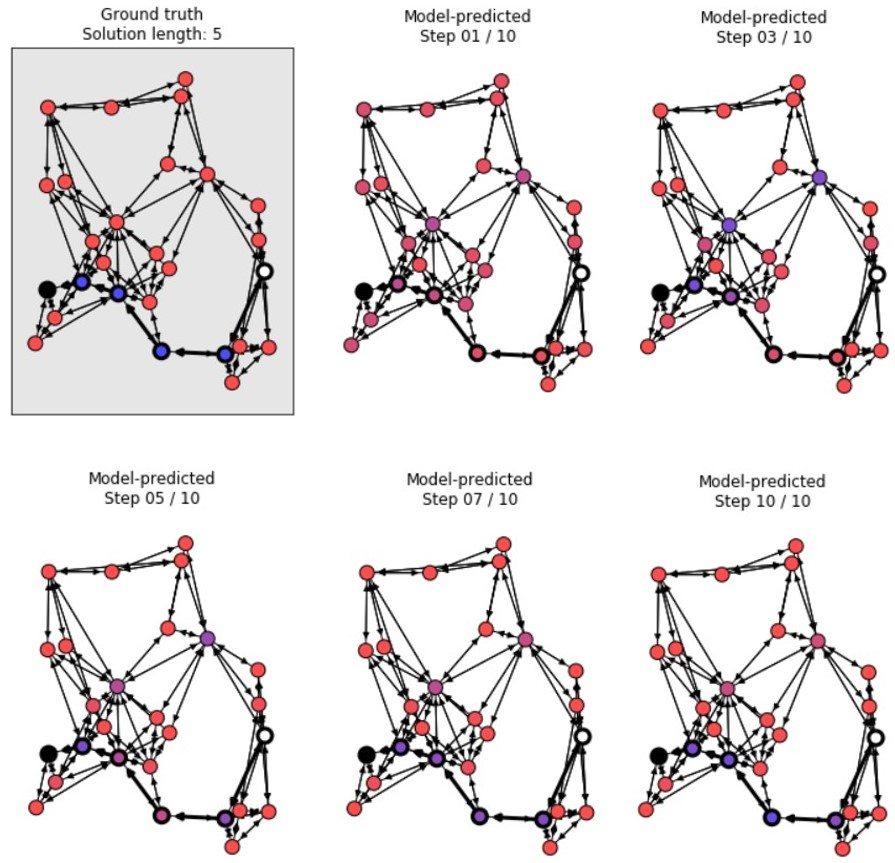
\includegraphics[scale=.6]{images/shortest_path_resolution.jpg}
    \caption{The ground truth for the shortest path between the white and the black nodes, and the different steps processed by the GNN. Blue corresponds to a high probability of being in the path, whereas red coresponds to a low probability.}
    \label{fig:shortest-path-resolution}
\end{figure}

    \subsection{Applications}
    \label{subsec:applications}

In this section, we just give a quick overview of the possible applications of GNNs. References are not given but can be found either in the aforementioned review \cite{wu2019comprehensive} or elsewhere.

\begin{itemize}
    \item \textbf{Computer Vision}. As many images are provided with a textual description, GNNs can be used in semantic segmentation or visual reasoning. Indeed, images can contain many objects and understanding the relationships between them helps characterize their interactions and can be very useful. It can also be used as an embedding block in an autoencoder network, such as U-Net. Another application concerns action recognition, where the joints of a skeleton naturally form a graph that can be used.
    
    \item \textbf{Physics and chemistry}. An interesting application is to predict the dynamics of physical systems, such as the mass-spring system mentioned previously. GNNs appear to perform much better than other models such as LSTMs (probably because of an "alignment" between a GNN and the task to solve). In chemistry, we already mentioned the example of predicting molecule properties with \cite{gilmer2017neural}.
    
    \item \textbf{Recommender systems}. A recommender system models relations between users or consumers and items. Its goal is to score the importance of an item to a user, which can be seen as an edge-level task.
    
    \item \textbf{Social network analysis}. Some papers have used GNNs in the context of influence maximization in a social network. It could also be used to study the contagion of nodes in a graph.
    
    \item \textbf{Programs correction}. A program coded in some language can also be seen as a graph with the different variables and functions. GNNs have been used for auto-completion or to correct code.
\end{itemize}

The range of applications is wide and this list is far from being complete, but it is here to give some examples.


\subsubsection*{Acknowledgments}

This review was done during a course given by Michal Valko for the Master Mathematics, Vision, Learning (MVA) from ENS Paris-Saclay, and was supervised by Claire Vernade and Rémy Degenne (warm thanks to them for their precious advices).

\medskip

\small

\bibliographystyle{unsrt}
\bibliography{report}


\end{document}
